% This LaTeX was auto-generated from an M-file by MATLAB.
% To make changes, update the M-file and republish this document.

\documentclass[12pt]{article}
\usepackage{natbib}
\usepackage[french]{babel}
\usepackage[utf8x]{inputenc}
\usepackage{lipsum}
\usepackage{amsmath}
\usepackage{graphicx}
\usepackage{hyperref}
\usepackage[final]{pdfpages}
\usepackage[T1]{fontenc}
\usepackage{listings}
\usepackage[colorinlistoftodos]{todonotes}
\usepackage{xcolor}
\usepackage[nottoc,numbib]{tocbibind}% Para que la bibliografia salga en el table of contents
\colorlet{Mycolor1}{green!10!orange!90!}
\usepackage{subfigure}
\sloppy
\definecolor{lightgray}{gray}{0.5}
\setlength{\parindent}{0pt}
\setlength{\parskip}{1em}

\bibliographystyle{abbrv}

\begin{document}
\title{Doc}
\author{CHIRINO CAICEDO Melet}
\begin{titlepage}

\newcommand{\HRule}{\rule{\linewidth}{0.5mm}} % Defines a new command for the horizontal lines, change thickness here

\center % Center everything on the page
 
%----------------------------------------------------------------------------------------
%	HEADING SECTIONS
%----------------------------------------------------------------------------------------

\textsc{\LARGE Université Toulouse III}\\[0.5cm] % Name of your university/college
\textsc{\Large Paul Sabatier}\\[1.0cm] % Major heading such as course name
\textsc{\large Projet VHDL-AMS M2 EEA}\\[0.5cm] % Minor heading such as course title

%----------------------------------------------------------------------------------------
%	TITLE SECTION
%----------------------------------------------------------------------------------------

\HRule \\[0.4cm]
{ \huge \bfseries Modélisation d'un système de freinage équipé d'un ABS }\\[0.4cm] % Title of your document
\HRule \\[1.5cm]
 
%----------------------------------------------------------------------------------------
%	AUTHOR SECTION
%----------------------------------------------------------------------------------------

\begin{minipage}{0.4\textwidth}
\begin{flushleft} \large
\markboth{Proyecto en \LaTeX}
\emph{Auteurs:}\\
\textsc{BEROY} Juan \\ % Your name
\textsc{CHIRINO} Melet % Your name
\end{flushleft}
\end{minipage}
~
\begin{minipage}{0.5\textwidth}
\begin{flushright} \large
\emph{Professor:} \\
\textsc{JAMMES} Bruno  % Supervisor's Name
\end{flushright}
\end{minipage}\\[2cm]

% If you don't want a supervisor, uncomment the two lines below and remove the section above
%\Large \emph{Author:}\\
%John \textsc{Smith}\\[3cm] % Your name

%----------------------------------------------------------------------------------------
%	DATE SECTION
%----------------------------------------------------------------------------------------

{\large \today}\\[2cm] % Date, change the \today to a set date if you want to be precise

%----------------------------------------------------------------------------------------
%	LOGO SECTION
%----------------------------------------------------------------------------------------


\includegraphics[width=5in]{images/Logo_UT32.jpg}\\[2cm] % Include a department/university logo - this will require the graphicx package
 
%----------------------------------------------------------------------------------------

\vfill % Fill the rest of the page with whitespace

\end{titlepage}

%\{Contents}
\tableofcontents
\newpage
\section{Simulation d’un système de freinage sans ABS}
\begin{par}
Construisez et validez le système de freinage, en assemblant les modèles VHDL-AMS du maître-cylindre de frein (2+3), de l’étrier de frein, de la roue et du ¼ de véhicule fournis. Le code se trouve dans l'annexe \ref{anexe:assemblage}. Sur la figure \ref{fig:assemblagepng} on peut voir graphiquement l'assemblage fait au debut.
\end{par}

\begin{figure}[!htb]
     \centering
     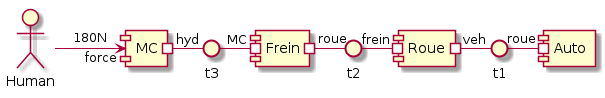
\includegraphics[width=\textwidth]{images/assemblage.png}
     \caption{Mod\`ele de l'assemblage.}
     \label{fig:assemblagepng}
\end{figure}

\begin{par}
Sur la figure \ref{fig:assemblage} on peut voir la vitesse du véhicule et comment il freine avec une force de $180N$ apliqu\'ee. Le temps de freinage est un peu apr\`es $3.5s$.
\end{par}
\begin{figure}[!htb]
     \centering
     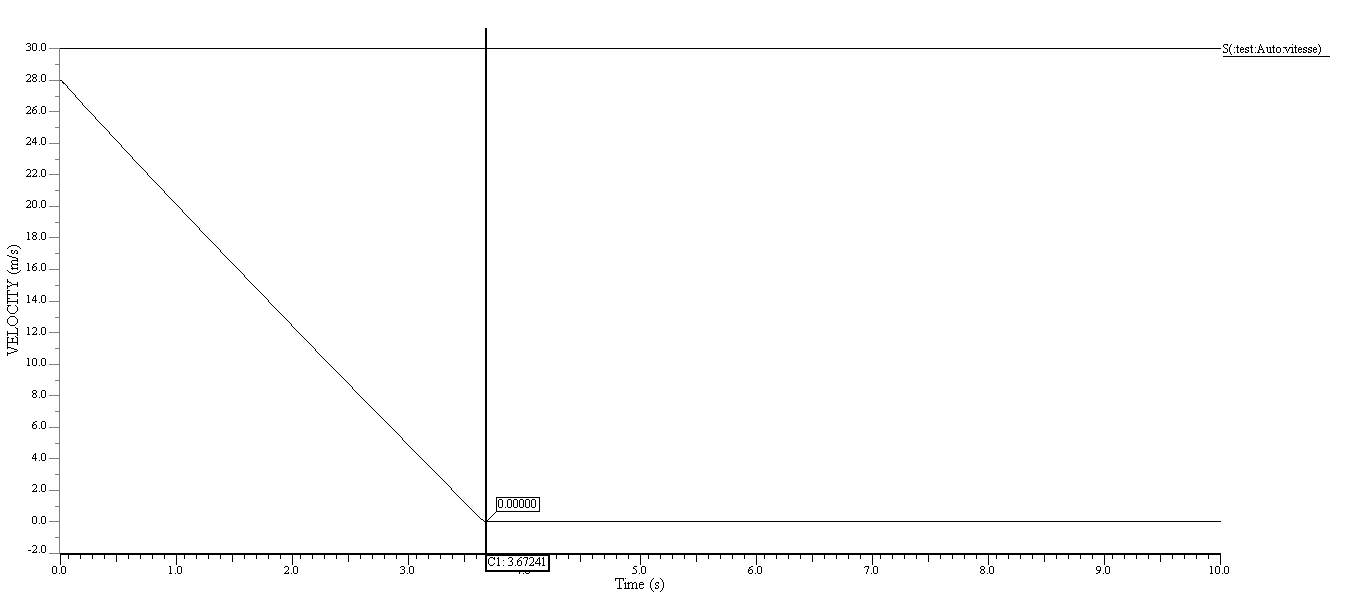
\includegraphics[width=\textwidth]{images/1-assemblage-done.png}
     \caption{Vitesse du mod\`ele de l'assemblage complet.}
     \label{fig:assemblage}
\end{figure}
 \subsection{Simulation sur sol sec}
Effectuer ensuite une simulation du système sur sol sec lorsque la vitesse initiale du véhicule est de 100km/h (environ 28 m/s) et qu’à t = 100ms le conducteur exerce un effort de 180N sur la pédale de frein avec un temps d’établissement de la force de 0.5s, et ce jusqu’à l’arrêt du véhicule.

\begin{par}
Sur la figure \ref{fig:q1-seche} on peut voir comment la voiture freine avec un peu de retard en comparaison avec la simulation de la figure \ref{fig:assemblage}. Le temps total de freinage ici cest $\approx 4.8$.
\end{par}

\begin{figure}[!htb]
     \centering
     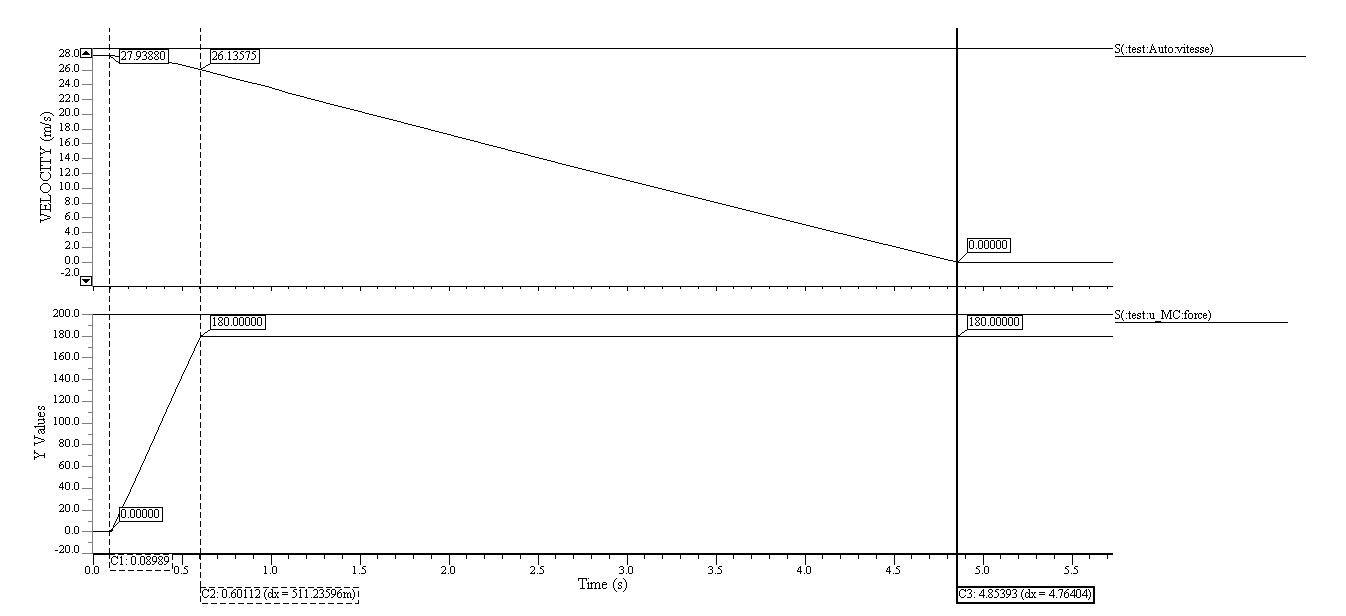
\includegraphics[width=\textwidth]{images/1-force-raw-seche.png}
     \caption{Simulation de freinage sur sol sèche.
    1) Vitesse du véhicule.
    2) Condition de freinage.}
     \label{fig:q1-seche}
\end{figure}

\subsection{Simulation sur sol humide}
 \begin{figure}
     \centering
     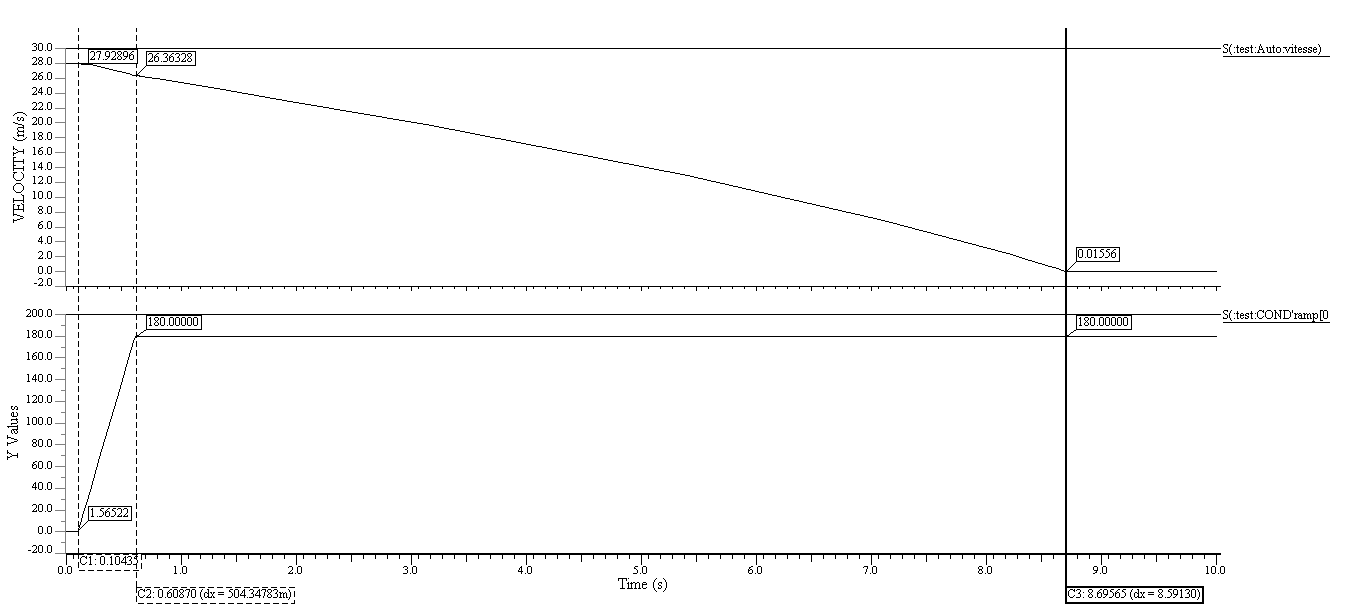
\includegraphics[width=\textwidth]{images/1-force-cond-humide.png}
     \caption{Simulation de freinage sur sol humide.
          1) Vitesse du véhicule.
     2) Condition de freinage.}
     \label{fig:q1-humide}
\end{figure}

\begin{par}
Il est évident que sur le sol sèche la voiture freine beaucoup plus rapidement que sur un sol humide, environ deux fois plus vite. En plus, la courbe de la figure \ref{fig:q1-humide} est moins linéaire que la figure \ref{fig:q1-seche}.
\end{par}

\section{Modélisation du système de freinage équipé d’un ABS}


\begin{par}
Pour construire le modelé nous avons du calculer le coefficient de glissement avec la formule suivante : 
\end{par}
\begin{equation}
    S = \frac{V_V - R*\Omega}{V_V}
\end{equation}
\begin{par}
Avec : 
\end{par}
\begin{itemize}
    \item $\Omega$ : Vitesse angulaire de la roue. \item $V_V$ : Vitesse du véhicule.
    \item $R$ : Rayon de la roue.
\end{itemize}
Et les conditions sont les suivantes : 
\begin{itemize}
    \item Réduire la pression en sortie du limiteur de pression en diminuant de $0.5V$ sa tension de commande si le glissement est supérieur a $50\%$.
    \item Rétablir la pression en sortie du régulateur en augmentant de $0.1V$ la tension de commande du limiteur si le glissement est inférieur a $50\%$.
\end{itemize}

\begin{par}
Le code se trouve sur l'annexe \ref{anexe:calculateur} et la figure \ref{fig:assemblage-abs} montre le montage fait. 
\end{par}

\begin{figure}[!htb]
     \centering
     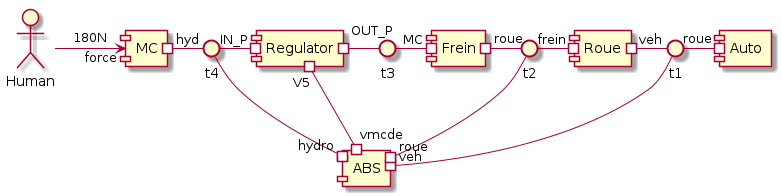
\includegraphics[width=\textwidth]{images/assemblage_abs.png}
     \caption{Mod\`ele avec calculateur ABS.}
     \label{fig:assemblage-abs}
\end{figure}
\begin{par}
Le sujet nous demande faire deux simulations pour voire le comportement du calculateur ABS dans une  situation de freinage réelle. Dans ces simulations nous n'allons utiliser que le sol mouill\'e parce que avec le sol sec le coeff de glissement calcul\'e n'atteint pas le seuil pour demarrer le fonctionement de l'ABS. La troisieme courbe de la figure \ref{fig:q22-seche} montre comment la valeur de l'abs ne change pas sur le sol sec.
\end{par}
 \begin{figure}
     \centering
     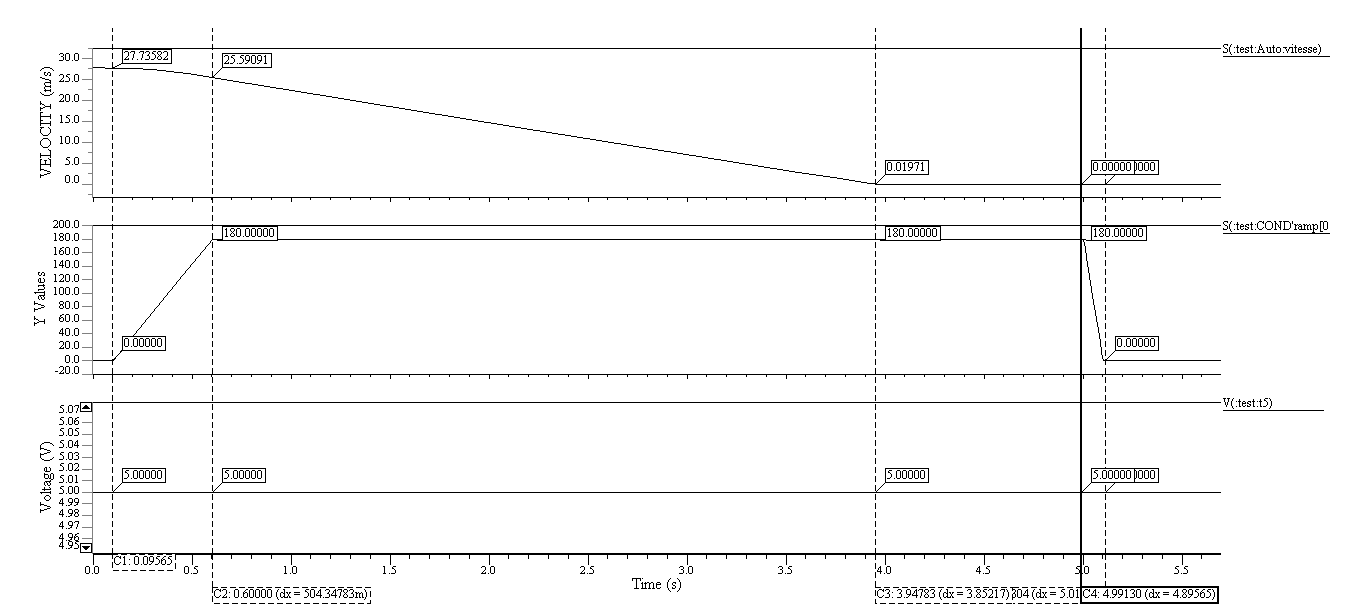
\includegraphics[width=\textwidth]{images/2-relache-seche.png}
     \caption{Simulation de freinage sur sol sec.      1) Vitesse du véhicule.
     2) Pression corrig\'ee sur le freine.
     3) Condition de freinage.}
     \label{fig:q22-seche}
\end{figure}
\subsection{Teste avec force constant}
\begin{par}
Le conducteur appui sur la pédale de frein (180 N) à t = 100ms, avec un temps d’établissement de la force de 0.5s, jusqu’à l’arrêt du véhicule. La vitesse initiale du véhicule est toujours de 100km/h. Comparer la distance d’arrêt avec celle obtenue sans antiblocage. Sur la figure \ref{fig:q2-humide} se montrent les résultats de ce simulation.
\end{par}

 \begin{figure}
     \centering
     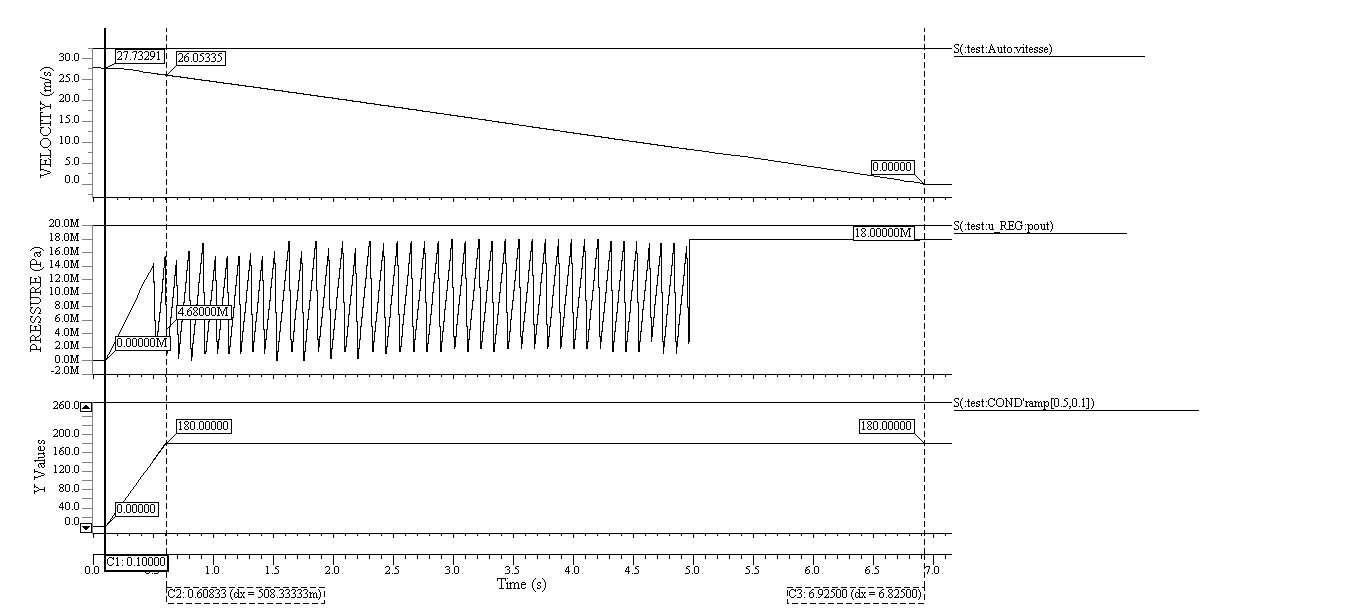
\includegraphics[width=\textwidth]{images/2-force-humide.png}
     \caption{Simulation de freinage sur sol humide.
     1) Vitesse du vehicule.
     2) Pression corrig\'ee sur le freine.
     3) Condition de freinage.}
     \label{fig:q2-humide}
\end{figure}
\begin{par}
On peut voir clairement (fig. \ref{fig:q2-humide}) comment la correction de pression sur le frein commence a se faire a partir d'un certain force apliqu\'ee par l'utilisateur et il commence \`a osciller pour éviter le blocage de la roue. Bien sur cela prend plus de temps mais le blocage de la roue peut finir par un évènement catastrophique.
\end{par}
\subsection{Teste avec relâchement du frein}
\begin{par}
Le conducteur appui sur la pédale de frein (180 N) à t = 100ms, avec un temps d’établissement de la force de 0.5s, puis relâche la pédale à t =5s, avec un temps d’annulation de la force de 100 ms. Vérifiez l’arrêt de l’antiblocage après le relâchement de la pédale.
\end{par}

 \begin{figure}
     \centering
     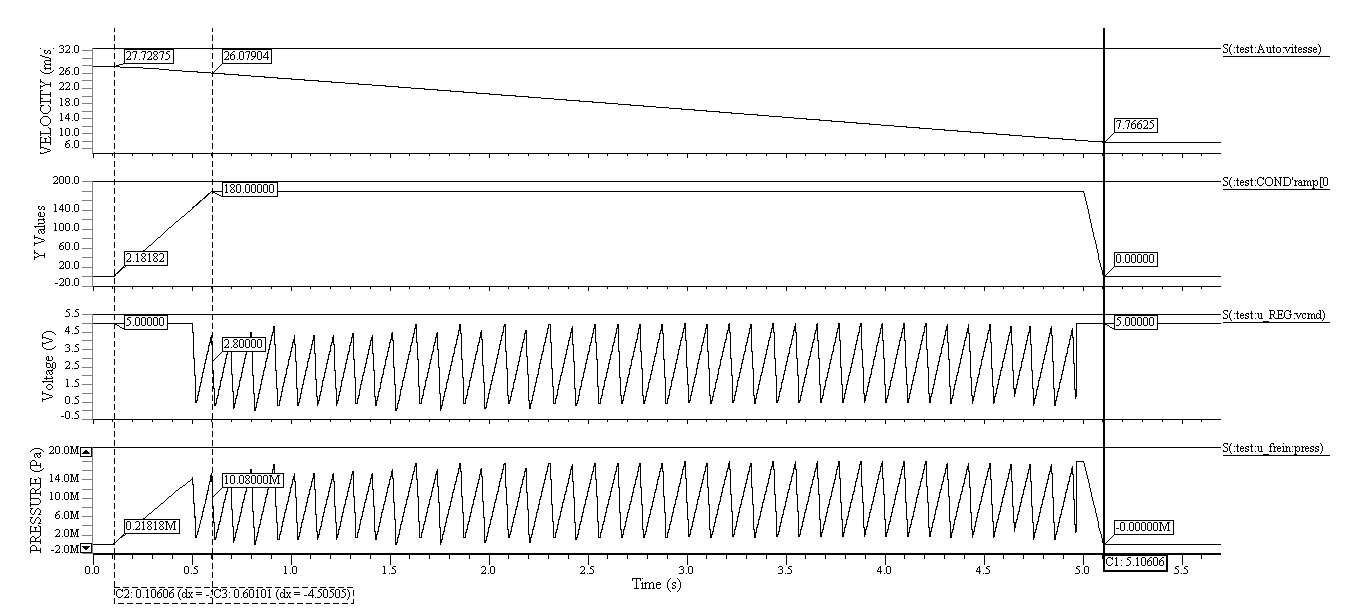
\includegraphics[width=\textwidth]{images/2-relache-humide.png}
     \caption{Simulation de freinage sur sol humide
     1) Vitesse lineaire du vehicule
     2) Profil de freinage
     3) Tension de commande du calculateur AB
     4) Presion corrig\'ee sur le frein}
     \label{fig:q22-humide}
\end{figure}

\begin{par}
Le profil de freinage se voit sur la deuxième courbe de la figure \ref{fig:q22-humide}, clairement le conducteur relâche la pédale. Les dernières traces nous montrent la tension de commande du calculateur ABS et la correction fait \`a partir de ce tension fait sur le frein pour éviter le blocage de la roue. \`A différence de la simulation de la figure \ref{fig:q2-humide} on voir comment la tension de commande du calculateur ABS d'arrêt apr\`es le relâchement de la pédale. Le code utilis\'e pour cette simulation se trouve sur l'annexe \ref{anexe:assemblage-abs-profil}.
\end{par}
\section{Intégration simplifiée du moteur thermique }
\begin{par}
Modifier le modèle global pour intégrer le couple généré par le moteur thermique. Simuler le comportement du système lorsque le conducteur accélère (couple moteur ramené sur la roue = 900 N.m pendant 2s, puis 500 N.m pendant 3s, puis 300 N.m pendant 4s) puis freine comme dans le test décrit au II-2. Le mod\`ele graphique de ce simulation se montre sur la figure \ref{fig:assemblage-abs-moteur} et la simulation sur les courbes de figure \ref{fig:q3-humide}. Le code utilis\'e pour cette simulation est sur l'annexe \ref{anexe:assemblage-abs-moteur}.
\end{par}

\begin{figure}[!htb]
     \centering
     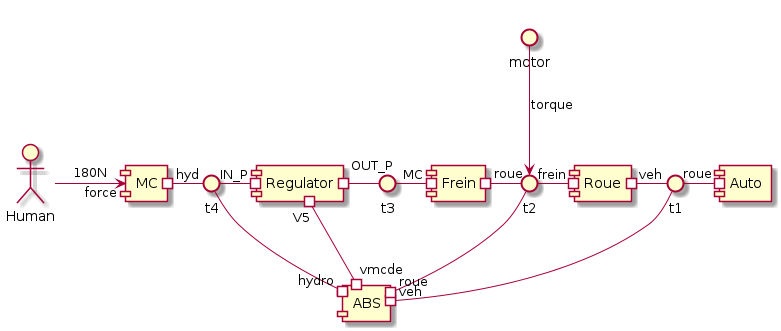
\includegraphics[width=\textwidth]{images/assemblage-moteur.png}
     \caption{Mod\`ele avec calculateur ABS et moteur thermique.}
     \label{fig:assemblage-abs-moteur}
\end{figure}

\begin{par}
On voit comment la vitesse du vehicule augmente pendant que le moteur accelere, et presque depuis le debut du freinage le calculateur ABS commence \`a faire eviter le blocage de la roue. Dans cette simulation nous avons inclus la vitesse rotational de la roue pour voire comment elle change avec la correction de l'ABS. Malheureusement la simulation de dure que 10s donc on ne peut pas voir plus loin mais les resultats seront les obtenus en simulations precedentes.
\end{par}

 \begin{figure}[!htb]
     \centering
     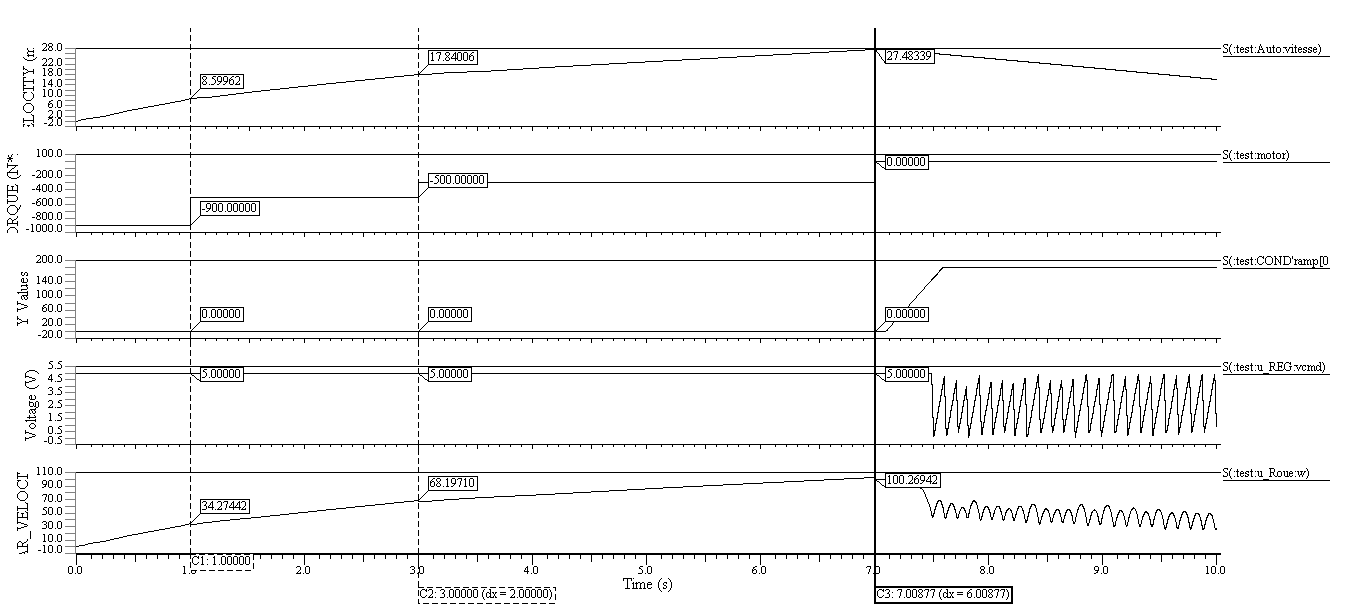
\includegraphics[width=\textwidth]{images/3-humide-cursors.png}
     \caption{1) Vitesse du vehicule
     2) Acceleration du moteur thermique
     3) Freine
     4) Tension de commande de l'ABS
     5) Vitesse angulaire de la roue}
     \label{fig:q3-humide}
\end{figure}

\newpage
\section{Annexes}
\begin{par}
Toutes les fichiers de ce projet se trouvent sur github : \url{https://github.com/MeletChirino/vhdl_ams}
No cars were harmed durign this simulations
\end{par}

\subsection{Code de l'assemblage complet}
\label{anexe:assemblage}
\begin{verbatim}
library ieee;
use ieee.mechanical_systems.all;
use ieee.fluidic_systems.all;
use ieee.math_real.all;
use ieee.electrical_systems.all;

use work.MES_TYPES.all;
use work.MES_CONSTANTES.all;

entity test is
    constant m_veh : MASS := 1500.0;
end test;

architecture behavioral of test is 
    terminal t1 : translational_velocity;
    terminal t2 : rotational_velocity;
    terminal t3 : fluidic;
    quantity f :FORCE := 180.0;
begin 

f==180.0;

Auto: 	entity vehicule(one) generic map (
        m=>m_veh,
        cx=>0.3,
        S=>1.8,
        v_init=>28.0
        ) 
    port map(roue=>t1);

u_Roue:  entity roue(A) generic map(
        route=>seche,
        m=>m_veh, 
        rR=>0.275, 
        IR=>0.4, 
        mu0_D=>1.0, 
        As=>0.01, 
        mu0_W=>0.5, 
        Vc=>27.8
        )
    port map(veh=>t1, frein => t2);

u_frein:  entity frein(one) generic map (
        coef_fric=>0.36,
        S=>1.0e-3, 
        R=>0.12
        )
    port map(MC=>t3, roue => t2);

u_MC:  entity maitre_cylindre(one) generic map (
        S=>1.0e-4,
        coef_assistance=>10.0
        )
    port map(hyd=>t3, force => f);

end behavioral; 
\end{verbatim}

\subsection{Calculateur ABS}
\label{anexe:calculateur}
\begin{verbatim}
library ieee;
use ieee.mechanical_systems.all;
use ieee.fluidic_systems.all;
use ieee.electrical_systems.all;
use ieee.std_logic_1164.all;

entity Calc_ABS is
    port(
        terminal veh : translational_velocity;
        terminal roue : rotational_velocity;
        terminal hydro : fluidic;
        terminal vcmde : electrical
    );
end Calc_ABS;

architecture simple of Calc_ABS is
	signal clk	: std_logic := '0';
	signal vcom     : real := 5.0;
	signal g : real;
	quantity vv across ii through vcmde;
	quantity pin across din through hydro;
	quantity vit across force through veh;
	quantity omega across tq through roue;
begin
        clk <= not clk after 1 ms;
        vv == vcom;  
        break on vcom; 
        din == 0.0;
        force == 0.0;
        tq == 0.0;
    process(clk)
    	variable S	: real; --coeff glisement
    	begin 
    		if (clk'event and clk = '1') then -- detect rising edge 
    			--if trasnlational speed under 30 adjust abs
    			if (vit > 8.3) then 
    			    --calculs coeff glissement
    				S := (vit - omega * 0.275) / vit; 
    				if(S >= 0.5) then 
    					if vcom > 0.5 then 
    						vcom <= vcom - 0.5;
    						end if; 
    				elsif (S < 0.5) then
    					if vcom < 4.9 then 
    						vcom <= vcom + 0.1;
    						end if;
    					end if; 
    			elsif(vit < 8.3 and vit >  0.0) then 
    				vcom <= 5.0;
    				end if;
    			if (pin = 0.0) then
    				vcom <= 5.0;
    				end if;
    			end if;
    			g<=S;
    		end process;
    end simple;
\end{verbatim}

\subsection{Code de l'assemblage complet avec calculateur ABS}
\label{anexe:assemblage-abs}
\begin{verbatim}
library ieee;
use ieee.mechanical_systems.all;
use ieee.fluidic_systems.all;
use ieee.math_real.all;
use ieee.electrical_systems.all;

use work.MES_TYPES.all;
use work.MES_CONSTANTES.all;

entity test is
    constant m_veh : MASS := 1500.0;
end test;

architecture I of test is 
    terminal t1 : translational_velocity;
    terminal t2 : rotational_velocity;
    terminal t3 : fluidic;
    terminal t4 : fluidic; 
    terminal t5 : electrical; 
    quantity f :FORCE := 180.0;
    signal COND :real := 0.0;
begin 

cond <= 180.0 after 100 ms;
f==cond'ramp(0.5, 0.1);
break on cond;

Auto: 	entity vehicule(one) generic map (
        m=>m_veh,
        cx=>0.3,
        S=>1.8,
        v_init=>27.8
        ) 
    port map(roue=>t1);

u_Roue:  entity roue(A) generic map(
        route=>humide,
        m=>m_veh, rR=>0.275,
        IR=>0.4,
        mu0_D=>1.0,
        As=>0.01,
        mu0_W=>0.5,Vc=>27.8
        )
    port map(veh=>t1, frein => t2);

u_frein:  entity frein(one) generic map (
        coef_fric=>0.36,
        S=>1.0e-3,
        R=>0.12
        )
    port map(MC=>t3, roue => t2);

u_MC:  entity maitre_cylindre(one) generic map (
        S=>1.0e-4,
        coef_assistance=>10.0
        )
    port map(hyd=>t4, force => f);

u_REG:  entity regulateur(one) generic map (
        P=>1.0e-4,
        tau=>10.0
        )
    port map(IN_P=>t4, OUT_P => t3, V => t5);

u_ABS:  entity Calc_ABS(simple) port map(
        veh => t1,
        roue => t2,
        hydro => t4,
        vcmde => t5
        );

end I; 
\end{verbatim}

\subsection{Code de l'assemblage complet avec calculateur ABS avec relachement du frein}
\label{anexe:assemblage-abs-profil}
\begin{verbatim}
library ieee;
use ieee.mechanical_systems.all;
use ieee.fluidic_systems.all;
use ieee.math_real.all;
use ieee.electrical_systems.all;

use work.MES_TYPES.all;
use work.MES_CONSTANTES.all;

entity test is
    constant m_veh : MASS := 1500.0;
end test;

architecture I of test is 
    terminal t1 : translational_velocity;
    terminal t2 : rotational_velocity;
    terminal t3 : fluidic;
    terminal t4 : fluidic; 
    terminal t5 : electrical; 
    quantity f :FORCE := 180.0;
    signal COND :real := 0.0;
begin 

cond <= 180.0 after 100 ms, 0.0 after 5000 ms;
f==cond'ramp(0.5);
break on cond;

Auto: 	entity vehicule(one) generic map (
        m=>m_veh,
        cx=>0.3,
        S=>1.8,
        v_init=>27.8
        ) 
    port map(roue=>t1);

u_Roue:  entity roue(A) generic map(
        route=>humide,
        m=>m_veh, rR=>0.275,
        IR=>0.4,
        mu0_D=>1.0,
        As=>0.01,
        mu0_W=>0.5,Vc=>27.8
        )
    port map(veh=>t1, frein => t2);

u_frein:  entity frein(one) generic map (
        coef_fric=>0.36,
        S=>1.0e-3,
        R=>0.12
        )
    port map(MC=>t3, roue => t2);

u_MC:  entity maitre_cylindre(one) generic map (
        S=>1.0e-4,
        coef_assistance=>10.0
        )
    port map(hyd=>t4, force => f);

u_REG:  entity regulateur(one) generic map (
        P=>1.0e-4,
        tau=>10.0
        )
    port map(IN_P=>t4, OUT_P => t3, V => t5);

u_ABS:  entity Calc_ABS(simple) port map(
        veh => t1,
        roue => t2,
        hydro => t4,
        vcmde => t5
        );

end I; 
\end{verbatim}

\subsection{Fichier de test}
\label{anexe:assemblage-abs-moteur}
\begin{verbatim}
library ieee;
use ieee.mechanical_systems.all;
use ieee.fluidic_systems.all;
use ieee.math_real.all;
use ieee.electrical_systems.all;

use work.MES_TYPES.all;
use work.MES_CONSTANTES.all;

entity test is
    constant m_veh : MASS := 1500.0;
end test;

architecture J of test is 
    terminal t1 : translational_velocity;
    terminal t2 : rotational_velocity;
    terminal t3 : fluidic;
    terminal t4 : fluidic; 
    terminal t5 : electrical; 
    quantity f :FORCE := 180.0;
    quantity motor through t2;
    signal COND :real := 0.0;
    signal torque : real := 0.0; 
begin 
cond <= 180.0 after 7100 ms, 0.0 after 12000 ms;
f==cond'ramp(0.5, 0.1);
	torque 	<= -900.0 after 0 ms,
			-500.0 after 1000 ms,
			-300.0 after 3000 ms,
			0.0 after 7000 ms;
motor == torque; 
break on torque; 

Auto: 	entity vehicule(one) generic map (
        m=>m_veh,
        cx=>0.3,
        S=>1.8,
        v_init=>0.028
        ) 
    port map(roue=>t1);

u_Roue:  entity roue(A) generic map(
        route=>humide,
        m=>m_veh,
        rR=>0.275,
        IR=>0.4,
        mu0_D=>1.0,
        As=>0.01,
        mu0_W=>0.5,
        Vc=>27.8
        )
    port map(veh=>t1, frein => t2);

u_frein:  entity frein(one) generic map (
        coef_fric=>0.36,
        S=>1.0e-3,
        R=>0.12
        )
    port map(MC=>t3, roue => t2);

u_MC:  entity maitre_cylindre(one) generic map (
        S=>1.0e-4,
        coef_assistance=>10.0
        )
    port map(hyd=>t4, force => f);

u_REG:  entity regulateur(one) generic map (
        P=>1.0e-4,
        tau=>10.0
        )
    port map(IN_P=>t4, OUT_P => t3, V => t5);

u_ABS:  entity Calc_ABS(simple) port map(
        veh => t1,
        roue => t2,
        hydro => t4,
        vcmde => t5
        );
end J; 
\end{verbatim}

\subsection{Code avec le moteur thermique}
\label{anexe:test-cmd}
\begin{verbatim}
* /home/beroy/BE_VHDL_AMS_BEROY_CHIRINO/test.cmd input netlist
* Creation Date : Fri Nov 19 09:39:06% CET 2021 
*


.tran 0.1s 10s
* User minimum step definition
.option hmin=1e-12
* User integration method selection
.option trap
* User ELDO accuracy specification
.option eps=5e-3
* User ELDO accuracy specification
.option tuning=standard
.end
\end{verbatim}

% \begin{figure}
%     \centering
%     \includegraphics[height=\textheight]{Anexes/RadiacionSolar13 (1).pdf}
%     \caption{Caption}
%     \label{fig:radiacion}
% \end{figure}


% Plantilla para colocar muchas imagenes con un multiplot
%\begin{figure}[!htb]
%\centering
%\subfigure[]{\includegraphics [width=2.5in]{lab_2_vision_15.png}}
%\subfigure[]{\includegraphics [width=2.5in]{lab_2_vision_16.png}}
%\subfigure[]{\includegraphics [width=2.5in]{lab_2_vision_17.png}}
%\caption{Paleta de colores}
%\end{figure}

% Plantilla para poner una imagen cualquiera
%\begin{figure}[!htb]
%\centering
%
%\caption{Histograma de la imagen}
%\end{figure}

%\bibliography{Biblio}

\end{document}